\chapter{Filesystems}

\epigraph{TODO}{}

Filesystems are integral to modern computers. Filesystems not only deal with storing local files, they handle special devices that allow for safe communication between the kernel and user space. Filesystems also deal with failures, scalability, indexing, encryption, compression and performance


\section{Unix Filesystem Conventions}

In standard unix file systems: 

\begin{enumerate}

\item \keyword{.} represents the current directory
\item \keyword{..} represents the parent directory
\item \keyword{...} is NOT a valid representation of any directory (this not the grandparent directory). It \emph{could} however be the name of a file on disk.
\item \keyword{~} is the name of the home directory usually
\end{enumerate}

\subsection{Pathing}

Absolute paths are paths that start from the `root node' of your directory tree. Relative paths are paths that start from your current position in the tree. If you start in your home directory ("~" for short), then \keyword{Desktop/cs241} would be a relative path. Its absolute path counterpart might be something like \keyword{/Users/[yourname]/Desktop/cs241}.

\subsection{\texorpdfstring{How do I simplify \texttt{a/b/../c/./}?}{How do I simplify a/b/../c/./?}}\label{how-do-i-simplify-ab..c.}

Paths are continually getting simplified too it is possible to have a path called \texttt{a/b/../c/./} and you can ask the filesystem to compress the path or get the realpath. To simplify by hand remember that \keyword{..} means `parent folder' and that \keyword{.} means `current folder'.

\begin{enumerate}
  \item \keyword{cd a} (in a) 
  Step 2: \keyword{cd b} (in a/b)
  Step 3: \keyword{cd ..} (in a, because .. represents `parent folder')
  Step 4: \keyword{cd c} (in a/c)
  Step 5: \keyword{cd .} (in a/c, because . represents `current folder')
\end{enumerate}

Thus, this path can be simplified to \keyword{a/c}.

\section{So what's a File System?}\label{so-whats-a-file-system}

A filesystem is how information is organized on disk. Whenever you want to access a file, the filesystem dictates how the file is read. Here is a sample image of a filesystem.

\begin{figure}[htbp]
\centering
\includegraphics{http://tinf2.vub.ac.be/~dvermeir/manual/uintro/disk.gif}
\caption{}
\end{figure}

Whoa that's a lot let's break it down * Superblock: This block contains metadata about the filesystem, how large, last modified time, a journal, number of inodes and the first inode start, number of data block and the first data block start. * Inode: This is the the key abstraction. An inode is a file. * Disk Blocks: These are where the data is stored. The actual contents of the file

\subsection{How does inode store the file contents?}\label{how-does-inode-store-the-file-contents}

\begin{figure}[htbp]
\centering
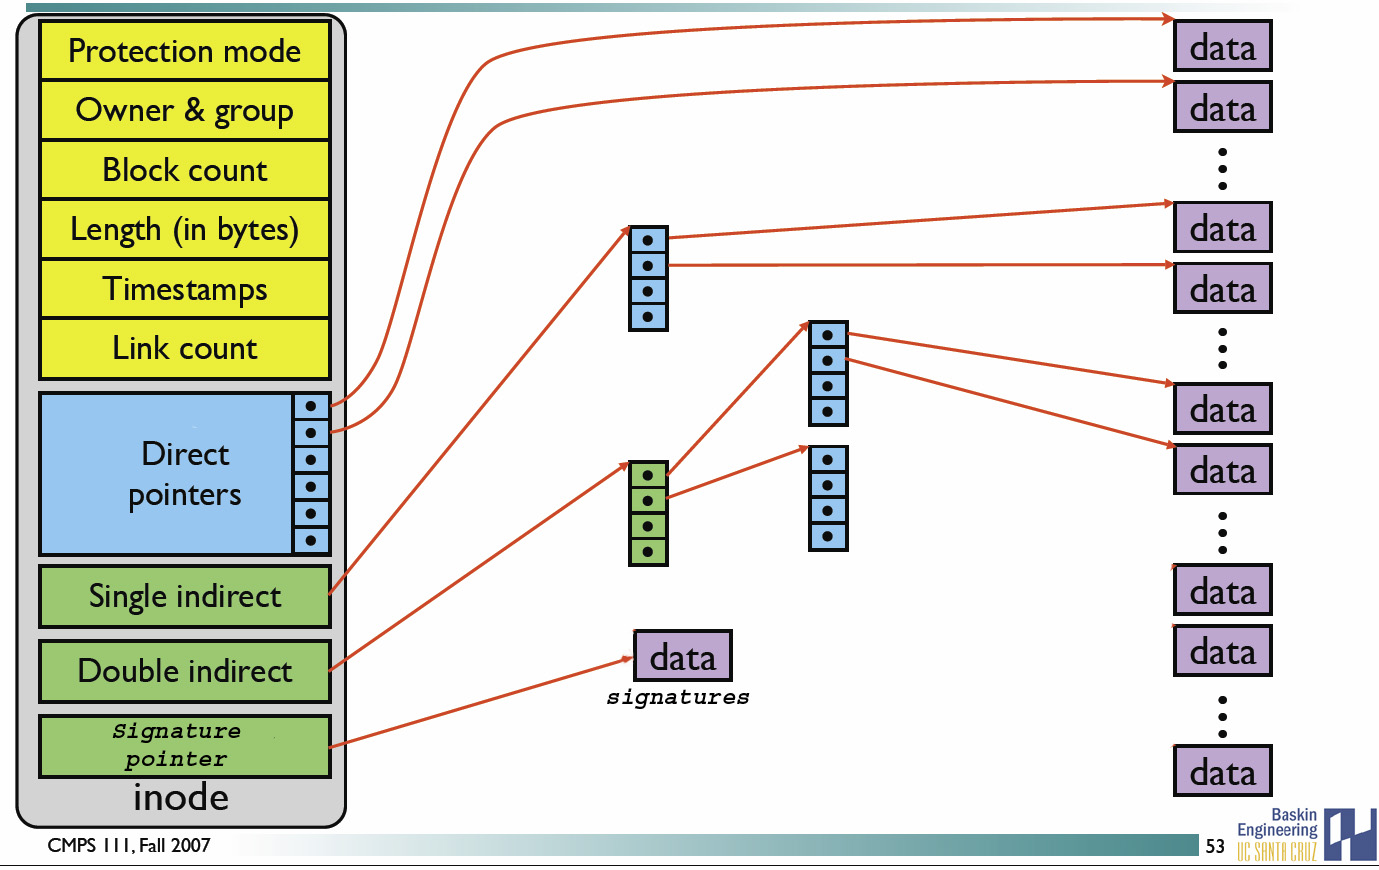
\includegraphics{https://classes.soe.ucsc.edu/cmps111/Fall08/inode_with_signatures.jpg}
\caption{}
\end{figure}

From \href{http://en.wikipedia.org/wiki/Inode}{Wikipedia}:

\begin{quote}
\emph{In a Unix-style file system, an index node, informally referred to as an inode, is a data structure used to represent a filesystem object, which can be one of various things including a file or a directory. Each inode stores the attributes and disk block location(s) of the filesystem object's data. Filesystem object attributes may include manipulation metadata (e.g.~change, access, modify time), as well as owner and permission data (e.g.~group-id, user-id, permissions).}
\end{quote}

To read the first few bytes of the file, follow the first direct block pointer to the first direct block and read the first few bytes, writing is the same process. If you want to read the entire file, keep reading direct blocks until your size runs out (we will talk about indirect blocks in a bit)

\begin{quote}
``All problems in computer science can be solved by another level of indirection.'' - David Wheeler
\end{quote}

\subsection{Why make disk blocks the same size as memory pages?}\label{why-make-disk-blocks-the-same-size-as-memory-pages}

To support virtual memory, so we can page stuff in and out of memory.

\subsection{What information do we want to store for each file?}\label{what-information-do-we-want-to-store-for-each-file}

\begin{itemize}
\tightlist
\item
  Filename
\item
  File size
\item
  Time created, last modified, last accessed
\item
  Permissions
\item
  Filepath
\item
  Checksum
\item
  File data (inode)
\end{itemize}

\subsection{What are the traditional permissions: user -- group -- other permissions for a file?}\label{what-are-the-traditional-permissions-user-group-other-permissions-for-a-file}

Some common file permissions include: * 755: \keyword{rwx r-x r-x}

user: \keyword{rwx}, group: \keyword{r-x}, others: \keyword{r-x}

User can read, write and execute. Group and others can only read and execute. * 644: \keyword{rw- r-- r--}

user: \keyword{rw-}, group: \keyword{r--}, others: \keyword{r--}

User can read and write. Group and others can only read.

\subsection{What are the the 3 permission bits for a regular file for each role?}\label{what-are-the-the-3-permission-bits-for-a-regular-file-for-each-role}

\begin{itemize}
\tightlist
\item
  Read (most significant bit)\\
\item
  Write (2nd bit)\\
\item
  Execute (least significant bit)
\end{itemize}

\subsection{\texorpdfstring{What do ``644'' ``755'' mean?}{What do 644 755 mean?}}\label{what-do-644-755-mean}

These are examples of permissions in octal format (base 8). Each octal digit corresponds to a different role (user, group, world).

We can read permissions in octal format as follows:\\
* 644 - R/W user permissions, R group permissions, R world permissions\\
* 755 - R/W/X user permissions, R/X group permissions, R/X world permissions

\subsection{How many pointers can you store in each indirection table?}\label{how-many-pointers-can-you-store-in-each-indirection-table}

As a worked example, suppose we divide the disk into 4KB blocks and we want to address up to 2\^{}32 blocks.

The maximum disk size is 4KB *2\^{}32 = 16TB (remember 2\^{}10 = 1024)

A disk block can store 4KB / 4B (each pointer needs to be 32 bits) = 1024 pointers. Each pointer refers to a 4KB disk block - so you can refer up to 1024*4KB = 4MB of data

For the same disk configuration, a double indirect block stores 1024 pointers to 1024 indirection tables. Thus a double-indirect block can refer up to 1024 * 4MB = 4GB of data.

Similarly, a triple indirect block can refer up to 4TB of data.

Big idea: Forget names of files: The `inode' is the file.

It is common to think of the file name as the `actual' file. It's not! Instead consider the inode as the file. The inode holds the meta-information (last accessed, ownership, size) and points to the disk blocks used to hold the file contents.

\subsection{So\ldots{} How do we implement a directory?}\label{so-how-do-we-implement-a-directory}

A directory is just a mapping of names to inode numbers. POSIX provides a small set of functions to read the filename and inode number for each entry (see below)

Let's think about what it looks like in the actual file system. Theoretically, directories are just like actual files. The disk blocks will contain \emph{directory entries} or \emph{dirents}. What that means is that our disk block can look like this

\textbar{} inode\_num \textbar{} name \textbar{} \textbar{}-----------\textbar{}------\textbar{} \textbar{} 2043567 \textbar{} hi.txt \textbar{} \ldots{}

Each directory entry could either be a fixed size, or a variable c-string. It depends on how the particular filesystem implements it at the lower level.

\subsection{How can I find the inode number of a file?}\label{how-can-i-find-the-inode-number-of-a-file}

From a shell, use \keyword{ls} with the \keyword{-i} option

\begin{lstlisting}
$ ls -i
12983989 dirlist.c      12984068 sandwich.c
\end{lstlisting}

From C, call one of the stat functions (introduced below).

\subsection{How do I find out meta-information about a file (or directory)?}\label{how-do-i-find-out-meta-information-about-a-file-or-directory}

Use the stat calls. For example, to find out when my `notes.txt' file was last accessed -

\begin{lstlisting}[language=C]
   struct stat s;
   stat("notes.txt", &s);
   printf("Last accessed %s", ctime(&s.st_atime));
\end{lstlisting}

There are actually three versions of \keyword{stat};

\begin{lstlisting}[language=C]
       int stat(const char *path, struct stat *buf);
       int fstat(int fd, struct stat *buf);
       int lstat(const char *path, struct stat *buf);
\end{lstlisting}

For example you can use \keyword{fstat} to find out the meta-information about a file if you already have an file descriptor associated with that file

\begin{lstlisting}[language=C]
   FILE *file = fopen("notes.txt", "r");
   int fd = fileno(file); /* Just for fun - extract the file descriptor from a C FILE struct */
   struct stat s;
   fstat(fd, & s);
   printf("Last accessed %s", ctime(&s.st_atime));
\end{lstlisting}

The third call `lstat' we will discuss when we introduce symbolic links.

In addition to access,creation, and modified times, the stat structure includes the inode number, length of the file and owner information.

\begin{lstlisting}[language=C]
struct stat {
               dev_t     st_dev;     /* ID of device containing file */
               ino_t     st_ino;     /* inode number */
               mode_t    st_mode;    /* protection */
               nlink_t   st_nlink;   /* number of hard links */
               uid_t     st_uid;     /* user ID of owner */
               gid_t     st_gid;     /* group ID of owner */
               dev_t     st_rdev;    /* device ID (if special file) */
               off_t     st_size;    /* total size, in bytes */
               blksize_t st_blksize; /* blocksize for file system I/O */
               blkcnt_t  st_blocks;  /* number of 512B blocks allocated */
               time_t    st_atime;   /* time of last access */
               time_t    st_mtime;   /* time of last modification */
               time_t    st_ctime;   /* time of last status change */
           };
\end{lstlisting}

\subsection{How do I list the contents of a directory ?}\label{how-do-i-list-the-contents-of-a-directory}

Let's write our own version of `ls' to list the contents of a directory.

\begin{lstlisting}[language=C]
#include <stdio.h>
#include <dirent.h>
#include <stdlib.h>
int main(int argc, char **argv) {
    if(argc == 1) {
        printf("Usage: %s [directory]\n", *argv);
        exit(0);
    }
    struct dirent *dp;
    DIR *dirp = opendir(argv[1]);
    while ((dp = readdir(dirp)) != NULL) {
        puts(dp->d_name);
    }

    closedir(dirp);
    return 0;
}
\end{lstlisting}

\subsection{How do I read the contents of a directory?}\label{how-do-i-read-the-contents-of-a-directory}

Ans: Use opendir readdir closedir For example, here's a very simple implementation of `ls' to list the contents of a directory.

\begin{lstlisting}[language=C]
#include <stdio.h>
#include <dirent.h>
#include <stdlib.h>
int main(int argc, char **argv) {
    if(argc ==1) {
        printf("Usage: %s [directory]\n", *argv);
        exit(0);
    }
    struct dirent *dp;
    DIR *dirp = opendir(argv[1]);
    while ((dp = readdir(dirp)) != NULL) {
        printf("%s %lu\n", dp-> d_name, (unsigned long)dp-> d_ino );
    }

    closedir(dirp);
    return 0;
}
\end{lstlisting}

Note: after a call to fork(), either (XOR) the parent or the child can use readdir(), rewinddir() or seekdir(). If both the parent and the child use the above, behavior is undefined.

\subsection{How do I check to see if a file is in the current directory?}\label{how-do-i-check-to-see-if-a-file-is-in-the-current-directory}

For example, to see if a particular directory includes a file (or filename) `name', we might write the following code. (Hint: Can you spot the bug?)

\begin{lstlisting}[language=C]
int exists(char *directory, char *name)  {
    struct dirent *dp;
    DIR *dirp = opendir(directory);
    while ((dp = readdir(dirp)) != NULL) {
        puts(dp->d_name);
        if (!strcmp(dp->d_name, name)) {
        return 1; /* Found */
        }
    }
    closedir(dirp);
    return 0; /* Not Found */
}
\end{lstlisting}

The above code has a subtle bug: It leaks resources! If a matching filename is found then `closedir' is never called as part of the early return. Any file descriptors opened, and any memory allocated, by opendir are never released. This means eventually the process will run out of resources and an \keyword{open} or \keyword{opendir} call will fail.

The fix is to ensure we free up resources in every possible code-path. In the above code this means calling \keyword{closedir} before \keyword{return 1}. Forgetting to release resources is a common C programming bug because there is no support in the C lanaguage to ensure resources are always released with all codepaths.

\subsection{What are the gotcha's of using readdir? For example to recursively search directories?}\label{what-are-the-gotchas-of-using-readdir-for-example-to-recursively-search-directories}

There are two main gotchas and one consideration: The \keyword{readdir} function returns ``.'' (current directory) and ``..'' (parent directory). If you are looking for sub-directories, you need to explicitly exclude these directories.

For many applications it's reasonable to check the current directory first before recursively searching sub-directories. This can be achieved by storing the results in a linked list, or resetting the directory struct to restart from the beginning.

One final note of caution: \keyword{readdir} is not thread-safe! For multi-threaded searches use \keyword{readdir_r} which requires the caller to pass in the address of an existing dirent struct.

See the man page of readdir for more details.

\subsection{How do I determine if a directory entry is a directory?}\label{how-do-i-determine-if-a-directory-entry-is-a-directory}

Ans: Use \keyword{S_ISDIR} to check the mode bits stored in the stat structure

And to check if a file is regular file use \keyword{S_ISREG},

\begin{lstlisting}[language=C]
   struct stat s;
   if (0 == stat(name, &s)) {
      printf("%s ", name);
      if (S_ISDIR( s.st_mode)) puts("is a directory");
      if (S_ISREG( s.st_mode)) puts("is a regular file");
   } else {
      perror("stat failed - are you sure I can read this file's meta data?");
   }
\end{lstlisting}

\subsection{Does a directory have an inode too?}\label{does-a-directory-have-an-inode-too}

Yes! Though a better way to think about this, is that a directory (like a file) \emph{is} an inode (with some data - the directory name and inode contents). It just happens to be a special kind of inode.

From \href{http://en.wikipedia.org/wiki/Inode}{Wikipedia}: \textgreater{} Unix directories are lists of association structures, each of which contains one filename and one inode number.

Remember, inodes don't contain filenames--only other file metadata.

\subsection{How can I have the same file appear in two different places in my file system?}\label{how-can-i-have-the-same-file-appear-in-two-different-places-in-my-file-system}

First remember that a file name != the file. Think of the inode as `the file' and a directory as just a list of names with each name mapped to an inode number. Some of those inodes may be regular file inodes, others may be directory inodes.

If we already have a file on a file system we can create another link to the same inode using the `ln' command

\begin{lstlisting}
$ ln file1.txt blip.txt
\end{lstlisting}

However blip.txt \emph{is} the same file; if I edit blip I'm editing the same file as `file1.txt!' We can prove this by showing that both file names refer to the same inode:

\begin{lstlisting}
$ ls -i file1.txt blip.txt
134235 file1.txt
134235 blip.txt
\end{lstlisting}

These kinds of links (aka directory entries) are called `hard links'

The equivalent C call is \keyword{link}

\begin{lstlisting}[language=C]
link(const char *path1, const char *path2);

link("file1.txt", "blip.txt");
\end{lstlisting}

For simplicity the above examples made hard links inside the same directory however hard links can be created anywhere inside the same filesystem.

\subsection{\texorpdfstring{What happens when I \texttt{rm} (remove) a file?}{What happens when I rm (remove) a file?}}\label{what-happens-when-i-rm-remove-a-file}

When you remove a file (using \keyword{rm} or \keyword{unlink}) you are removing an inode reference from a directory. However the inode may still be referenced from other directories. In order to determine if the contents of the file are still required, each inode keeps a reference count that is updated whenever a new link is created or destroyed.

\subsection{Case study: Back up software that minimizes file duplication}\label{case-study-back-up-software-that-minimizes-file-duplication}

An example use of hard-links is to efficiently create multiple archives of a file system at different points in time. Once the archive area has a copy of a particular file, then future archives can re-use these archive files rather than creating a duplicate file. Apple's ``Time Machine'' software does this.

\subsection{Can I create hard links to directories as well as regular files?}\label{can-i-create-hard-links-to-directories-as-well-as-regular-files}

No. Well yes. Not really\ldots{} Actually you didn't really want to do this, did you? The POSIX standard says no you may not! The \keyword{ln} command will only allow root to do this and only if you provide the \keyword{-d} option. However even root may not be able to perform this because most filesystems prevent it!

Why? The integrity of the file system assumes the directory structure (excluding softlinks which we will talk about later) is a non-cyclic tree that is reachable from the root directory. It becomes expensive to enforce or verify this constraint if directory linking is allowed. Breaking these assumptions can cause file integrity tools to not be able to repair the file system. Recursive searches potentially never terminate and directories can have more than one parent but ``..'' can only refer to a single parent. All in all, a bad idea.

\section{Remind Me What do Permissions mean again?}\label{remind-me-what-do-permissions-mean-again}

Every file and directory has a set of 9 permission bits and a type field * r, permission to read the file * w, permission to write to the file * x, permission to execute the file

chmod 777

\begin{longtable}[c]{@{}llll@{}}
\toprule
chmod & 7 & 7 & 7\tabularnewline
\midrule
\endhead
01 & 111 & 111 & 111\tabularnewline
d & rwx & rwx & rwx\tabularnewline
1 & 2 & 3 & 4\tabularnewline
\bottomrule
\end{longtable}

\begin{enumerate}
\def\labelenumi{\arabic{enumi}.}
\tightlist
\item
  Type of the file
\item
  Owner Permissions
\item
  Group Permissions
\item
  Everybody else's permission
\end{enumerate}

\keyword{mknod} changes the first field, the type of the file. \keyword{chmod} takes a number and a file and changes the permission bits.

The file has an owner. If your process has the same user id as the owner (or root) then the permissions in the first triad apply to you. If you are in the same group as the file (all files are also owned by a group) then the next set of permission bits applies to you. If none of the above apply, the last triad applies to you.

\subsection{How do I change the permissions on a file?}\label{how-do-i-change-the-permissions-on-a-file}

Use \keyword{chmod} (short for ``change the file mode bits'')

There is a system call, \keyword{int chmod(const char *path, mode_t mode);} but we will concentrate on the shell command. There's two common ways to use \keyword{chmod} ; with an octal value or with a symbolic string:

\begin{lstlisting}
$ chmod 644 file1
$ chmod 755 file2
$ chmod 700 file3
$ chmod ugo-w file4
$ chmod o-rx file4
\end{lstlisting}

The base-8 (`octal') digits describe the permissions for each role: The user who owns the file, the group and everyone else. The octal number is the sum of three values given to the three types of permission: read(4), write(2), execute(1)

Example: chmod 755 myfile * r + w + x = digit * user has 4+2+1, full permission * group has 4+0+1, read and execute permission * all users have 4+0+1, read and execute permission

\subsection{How do I read the permission string from ls?}\label{how-do-i-read-the-permission-string-from-ls}

Use `ls -l'. Note that the permissions will output in the format `drwxrwxrwx'. The first character indicates the type of file type. Possible values for the first character: * (-) regular file * (d) directory * (c) character device file * (l) symbolic link * (p) pipe * (b) block device * (s) socket

\subsection{What is sudo?}\label{what-is-sudo}

Use \keyword{sudo} to become the admin on the machine. e.g.~Normally (unless explicitly specified in the `/etc/fstab' file, you need root access to mount a filesystem). \keyword{sudo} can be used to temporarily run a command as root (provided the user has sudo privileges)

\begin{lstlisting}
$ sudo mount /dev/sda2 /stuff/mydisk
$ sudo adduser fred
\end{lstlisting}

\subsection{How do I change ownership of a file?}\label{how-do-i-change-ownership-of-a-file}

Use \keyword{chown username filename}

\subsection{How do I set permissions from code?}\label{how-do-i-set-permissions-from-code}

\keyword{chmod(const char *path, mode_t mode);}

\subsection{\texorpdfstring{Why are some files `setuid'? What does this mean?}{Why are some files setuid? What does this mean?}}\label{why-are-some-files-setuid-what-does-this-mean}

The set-user-ID-on-execution bit changes the user associated with the process when the file is run. This is typically used for commands that need to run as root but are executed by non-root users. An example of this is \keyword{sudo}

The set-group-ID-on-execution changes the group under which the process is run.

\subsection{Why are they useful?}\label{why-are-they-useful}

The most common usecase is so that the user can have root(admin) access for the duration of the program.

\subsection{What permissions does sudo run as ?}\label{what-permissions-does-sudo-run-as}

\begin{lstlisting}
$ ls -l /usr/bin/sudo
-r-s--x--x  1 root  wheel  327920 Oct 24 09:04 /usr/bin/sudo
\end{lstlisting}

The `s' bit means execute and set-uid; the effective userid of the process will be different from the parent process. In this example it will be root

\subsection{What's the difference between getuid() and geteuid()?}\label{whats-the-difference-between-getuid-and-geteuid}

\begin{itemize}
\tightlist
\item
  \keyword{getuid} returns the real user id (zero if logged in as root)
\item
  \keyword{geteuid} returns the effective userid (zero if acting as root, e.g.~due to the setuid flag set on a program)
\end{itemize}

\subsection{How do I ensure only privileged users can run my code?}\label{how-do-i-ensure-only-privileged-users-can-run-my-code}

\begin{itemize}
\tightlist
\item
  Check the effective permissions of the user by calling \keyword{geteuid()}. A return value of zero means the program is running effectively as root.
\end{itemize}

\subsection{How do I find out if file (an inode) is a regular file or directory?}\label{how-do-i-find-out-if-file-an-inode-is-a-regular-file-or-directory}

Use the \keyword{S_ISDIR} macro to check the mode bits in the stat struct:

\begin{lstlisting}[language=C]
struct stat s;
stat("/tmp", &s);
if (S_ISDIR(s.st_mode)) { ... 
\end{lstlisting}

Note, later we will write robust code to verify that the stat call succeeds (returns 0); if the \keyword{stat} call fails, we should assume the stat struct content is arbitrary.

\subsection{How do I recurse into subdirectories?}\label{how-do-i-recurse-into-subdirectories}

First a puzzle - how many bugs can you find in the following code?

\begin{lstlisting}[language=C]
void dirlist(char *path) {
  
  struct dirent *dp;
  DIR *dirp = opendir(path);
  while ((dp = readdir(dirp)) != NULL) {
     char newpath[strlen(path) + strlen(dp->d_name) + 1];
     sprintf(newpath,"%s/%s", newpath, dp->d_name);
     printf("%s\n", dp->d_name);
     dirlist(newpath);
  }
}

int main(int argc, char **argv) { dirlist(argv[1]); return 0; }
\end{lstlisting}

Did you find all 5 bugs?

\begin{lstlisting}[language=C]
// Check opendir result (perhaps user gave us a path that can not be opened as a directory
if (!dirp) { perror("Could not open directory"); return; }
// +2 as we need space for the / and the terminating 0
char newpath[strlen(path) + strlen(dp->d_name) + 2]; 
// Correct parameter
sprintf(newpath,"%s/%s", path, dp->d_name); 
// Perform stat test (and verify) before recursing
if (0 == stat(newpath,&s) && S_ISDIR(s.st_mode)) dirlist(newpath)
// Resource leak: the directory file handle is not closed after the while loop
closedir(dirp);
\end{lstlisting}

\subsection{What are symbolic links? How do they work? How do I make one?}\label{what-are-symbolic-links-how-do-they-work-how-do-i-make-one}

\begin{lstlisting}[language=C]
symlink(const char *target, const char *symlink);
\end{lstlisting}

To create a symbolic link in the shell use \keyword{ln -s}

To read the contents of the link as just a file use \keyword{readlink}

\begin{lstlisting}
$ readlink myfile.txt
../../dir1/notes.txt
\end{lstlisting}

To read the meta-(stat) information of a symbolic link use \keyword{lstat} not \keyword{stat}

\begin{lstlisting}[language=C]
struct stat s1, s2;
stat("myfile.txt", &s1); // stat info about  the notes.txt file
lstat("myfile.txt", &s2); // stat info about the symbolic link
\end{lstlisting}

\subsection{Advantages of symbolic links}\label{advantages-of-symbolic-links}

\begin{itemize}
\tightlist
\item
  Can refer to files that don't exist yet
\item
  Unlike hard links, can refer to directories as well as regular files
\item
  Can refer to files (and directories) that exist outside of the current file system
\end{itemize}

Main disadvantage: Slower than regular files and directories. When the links contents are read, they must be interpreted as a new path to the target file.

\subsection{\texorpdfstring{What is \texttt{/dev/null} and when is it used?}{What is /dev/null and when is it used?}}\label{what-is-devnull-and-when-is-it-used}

The file \keyword{/dev/null} is a great place to store bits that you never need to read! Bytes sent to \keyword{/dev/null/} are never stored - they are simply discarded. A common use of \keyword{/dev/null} is to discard standard output. For example,

\begin{lstlisting}
$ ls . >/dev/null
\end{lstlisting}

\subsection{Why would I want to set a directory's sticky bit?}\label{why-would-i-want-to-set-a-directorys-sticky-bit}

When a directory's sticky bit is set only the file's owner, the directory's owner, and the root user can rename (or delete) the file. This is useful when multiple users have write access to a common directory.

A common use of the sticky bit is for the shared and writable \keyword{/tmp} directory.

\subsection{\texorpdfstring{Why do shell and script programs start with \texttt{\#!/usr/bin/env\ python} ?}{Why do shell and script programs start with \#!/usr/bin/env python ?}}\label{why-do-shell-and-script-programs-start-with-usrbinenv-python}

Ans: For portability! While it is possible to write the fully qualified path to a python or perl interpreter, this approach is not portable because you may have installed python in a different directory.

To overcome this use the \keyword{env} utility is used to find and execute the program on the user's path. The env utility itself has historically been stored in \keyword{/usr/bin} - and it must be specified with an absolute path.

\subsection{\texorpdfstring{How do I make `hidden' files i.e.~not listed by ``ls''? How do I list them?}{How do I make hidden files i.e.~not listed by ls? How do I list them?}}\label{how-do-i-make-hidden-files-i.e.not-listed-by-ls-how-do-i-list-them}

Easy! Create files (or directories) that start with a ``.'' - then (by default) they are not displayed by standard tools and utilities.

This is often used to hide configuration files inside the user's home directory. For example \keyword{ssh} stores its preferences inside a directory called \keyword{.sshd}

To list all files including the normally hidden entries use \keyword{ls} with \keyword{-a} option

\begin{lstlisting}
$ ls -a
.           a.c         myls
..          a.out           other.txt
.secret 
\end{lstlisting}

\subsection{What happens if I turn off the execute bit on directories?}\label{what-happens-if-i-turn-off-the-execute-bit-on-directories}

The execute bit for a directory is used to control whether the directory contents is listable.

\begin{lstlisting}
$ chmod ugo-x dir1
$ ls -l
drw-r--r--   3 angrave  staff   102 Nov 10 11:22 dir1
\end{lstlisting}

However when attempting to list the contents of the directory,

\begin{lstlisting}
$ ls dir1
ls: dir1: Permission denied
\end{lstlisting}

In other words, the directory itself is discoverable but its contents cannot be listed.

\subsection{What is file globbing (and who does it)?}\label{what-is-file-globbing-and-who-does-it}

Before executing the program the shell expands parameters into matching filenames. For example, if the current directory has three filenames that start with my ( my1.txt mytext.txt myomy), then

\begin{lstlisting}
$ echo my*
\end{lstlisting}

Expands to

\begin{lstlisting}
$ echo my1.txt mytext.txt myomy
\end{lstlisting}

This is known as file globbing and is processed before the command is executed. ie the command's parameters are identical to manually typing every matching filename.

\subsection{Creating secure directories}\label{creating-secure-directories}

Suppose you created your own directory in /tmp and then set the permissions so that only you can use the directory (see below). Is this secure?

\begin{lstlisting}
$ mkdir /tmp/mystuff
$ chmod 700 /tmp/mystuff
\end{lstlisting}

There is a window of opportunity between when the directory is created and when it's permissions are changed. This leads to several vulnerabilities that are based on a race condition (where an attacker modifies the directory in some way before the privileges are removed). Some examples include:

Another user replaces \keyword{mystuff} with a hardlink to an existing file or directory owned by the second user, then they would be able to read and control the contents of the \keyword{mystuff} directory. Oh no - our secrets are no longer secret!

However in this specific example the \keyword{/tmp} directory has the sticky bit set, so other users may not delete the \keyword{mystuff} directory, and the simple attack scenario described above is impossible. This does not mean that creating the directory and then later making the directory private is secure! A better version is to atomically create the directory with the correct permissions from its inception -

\begin{lstlisting}
$ mkdir -m 700 /tmp/mystuff
\end{lstlisting}

\subsection{How do I automatically create parent directories?}\label{how-do-i-automatically-create-parent-directories}

\begin{lstlisting}
$ mkdir -p d1/d2/d3
\end{lstlisting}

Will automatically create d1 and d2 if they don't exist.

\subsection{My default umask 022; what does this mean?}\label{my-default-umask-022-what-does-this-mean}

The umask \emph{subtracts} (reduces) permission bits from 777 and is used when new files and new directories are created by open,mkdir etc. Thus \keyword{022} (octal) means that group and other privileges will not include the writable bit . Each process (including the shell) has a current umask value. When forking, the child inherits the parent's umask value.

For example, by setting the umask to 077 in the shell, ensures that future file and directory creation will only be accessible to the current user,

\begin{lstlisting}
$ umask 077
$ mkdir secretdir
\end{lstlisting}

As a code example, suppose a new file is created with \keyword{open()} and mode bits \keyword{666} (write and read bits for user,group and other):

\begin{lstlisting}[language=C]
open("myfile", O_CREAT, S_IRUSR | S_IWUSR | S_IRGRP | S_IWGRP | S_IROTH | S_IWOTH);
\end{lstlisting}

If umask is octal 022, then the permissions of the created file will be 0666 \& \textasciitilde{}022 ie.

\begin{lstlisting}[language=C]
           S_IRUSR | S_IWUSR | S_IRGRP | S_IROTH
\end{lstlisting}

\subsection{How can I copy bytes from one file to another?}\label{how-can-i-copy-bytes-from-one-file-to-another}

Use the versatile \keyword{dd} command. For example, the following command copies 1 MB of data from the file \keyword{/dev/urandom} to the file \keyword{/dev/null}. The data is copied as 1024 blocks of blocksize 1024 bytes.

\begin{lstlisting}
$ dd if=/dev/urandom of=/dev/null bs=1k count=1024
\end{lstlisting}

Both the input and output files in the example above are virtual - they don't exist on a disk. This means the speed of the transfer is unaffected by hardware power. Instead they are part of the \keyword{dev} filesystem, which is virtual filesystem provided by the kernel. The virtual file \keyword{/dev/urandom} provides an infinite stream of random bytes, while the virtal file \keyword{/dev/null} ignores all bytes written to it. A common use of \keyword{/dev/null} is to discard the output of a command,

\begin{lstlisting}
$ myverboseexecutable > /dev/null
\end{lstlisting}

Another commonly used /dev virtual file is \keyword{/dev/zero} which provides an infinite stream of zero bytes. For example, we can benchmark the operating system performance of reading stream zero bytes in the kernel into a process memory and writing the bytes back to the kernel without any disk I/O. Note the throughput (\textasciitilde{}20GB/s) is strongly dependent on blocksize. For small block sizes the overhead of additional \keyword{read} and \keyword{write} system calls will dominate.

\begin{lstlisting}
$ dd if=/dev/zero of=/dev/null bs=1M count=1024
1024+0 records in
1024+0 records out
1073741824 bytes (1.1 GB) copied, 0.0539153 s, 19.9 GB/s
\end{lstlisting}

\subsection{What happens when I touch a file?}\label{what-happens-when-i-touch-a-file}

The \keyword{touch} executable creates file if it does not exist and also updates the file's last modified time to be the current time. For example, we can make a new private file with the current time:

\begin{lstlisting}
$ umask 077       # all future new files will maskout all r,w,x bits for group and other access
$ touch file123   # create a file if it does not exist, and update its modified time
$ stat file123
  File: `file123'
  Size: 0           Blocks: 0          IO Block: 65536  regular empty file
Device: 21h/33d Inode: 226148      Links: 1
Access: (0600/-rw-------)  Uid: (395606/ angrave)   Gid: (61019/     ews)
Access: 2014-11-12 13:42:06.000000000 -0600
Modify: 2014-11-12 13:42:06.001787000 -0600
Change: 2014-11-12 13:42:06.001787000 -0600
\end{lstlisting}

An example use of touch is to force make to recompile a file that is unchanged after modifying the compiler options inside the makefile. Remeber that make is `lazy' - it will compare the modified time of the source file with the corresponding output file to see if the file needs to be recompiled

\begin{lstlisting}
$ touch myprogram.c   # force my source file to be recompiled
$ make
\end{lstlisting}

\subsection{Virtual file systems}\label{virtual-file-systems}

POSIX systems, such as Linux and Mac OSX (which is based on BSD) include several virtual filesystems that are mounted (available) as part of the file-system. Files inside these virtual filesystems do not exist on the disk; they are generated dynamically by the kernel when a process requests a directory listing. Linux provides 3 main virtual filesystems

\begin{lstlisting}
/dev  - A list of physical and virtual devices (for example network card, cdrom, random number generator)
/proc - A list of resources used by each process and (by tradition) set of system information
/sys - An organized list of internal kernel entities
\end{lstlisting}

For example if I want a continuous stream of 0s, I can \keyword{cat /dev/zero}.

\subsection{How do I find out what filesystems are currently available (mounted)?}\label{how-do-i-find-out-what-filesystems-are-currently-available-mounted}

Use \keyword{mount} Using mount without any options generates a list (one filesystem per line) of mounted filesystems including networked, virtual and local (spinning disk / SSD-based) filesystems. Here is a typical output of mount

\begin{lstlisting}
$ mount
/dev/mapper/cs241--server_sys-root on / type ext4 (rw)
proc on /proc type proc (rw)
sysfs on /sys type sysfs (rw)
devpts on /dev/pts type devpts (rw,gid=5,mode=620)
tmpfs on /dev/shm type tmpfs (rw,rootcontext="system_u:object_r:tmpfs_t:s0")
/dev/sda1 on /boot type ext3 (rw)
/dev/mapper/cs241--server_sys-srv on /srv type ext4 (rw)
/dev/mapper/cs241--server_sys-tmp on /tmp type ext4 (rw)
/dev/mapper/cs241--server_sys-var on /var type ext4 (rw)rw,bind)
/srv/software/Mathematica-8.0 on /software/Mathematica-8.0 type none (rw,bind)
engr-ews-homes.engr.illinois.edu:/fs1-homes/angrave/linux on /home/angrave type nfs (rw,soft,intr,tcp,noacl,acregmin=30,vers=3,sec=sys,sloppy,addr=128.174.252.102)
\end{lstlisting}

Notice that each line includes the filesystem type source of the filesystem and mount point. To reduce this output we can pipe it into \keyword{grep} and only see lines that match a regular expression.

\begin{lstlisting}
>mount | grep proc  # only see lines that contain 'proc'
proc on /proc type proc (rw)
none on /proc/sys/fs/binfmt_misc type binfmt_misc (rw)
\end{lstlisting}

\subsection{Differences between random and urandom?}\label{differences-between-random-and-urandom}

/dev/random is a file which contains number generator where the entropy is determined from environmental noise. Random will block/wait until enough entropy is collected from the environment.

/dev/urandom is like random, but differs in the fact that it allows for repetition (lower entropy threshold), thus wont block.

\subsection{Other Filesystems}\label{other-filesystems}

\begin{lstlisting}
$ cat /proc/sys/kernel/random/entropy_avail
$ hexdump /dev/random
$ hexdump /dev/urandom

$ cat /proc/meminfo
$ cat /proc/cpuinfo
$ cat /proc/cpuinfo | grep bogomips

$ cat /proc/meminfo | grep Swap

$ cd /proc/self
$ echo $$; cd /proc/12345; cat maps
\end{lstlisting}

\subsection{Mounting a filesystem}\label{mounting-a-filesystem}

Let's say I have a filesystem hooked up on \keyword{/dev/cdrom} that I want to read from. I have to mound it to a directory before I can do any operations.

\begin{lstlisting}
$ sudo mount /dev/cdrom /media/cdrom
$ mount
$ mount | grep proc
\end{lstlisting}

\subsection{How do I mount a disk image?}\label{how-do-i-mount-a-disk-image}

Suppose you had downloaded a bootable linux disk image\ldots{}

\begin{lstlisting}
wget http://cosmos.cites.illinois.edu/pub/archlinux/iso/2015.04.01/archlinux-2015.04.01-dual.iso
\end{lstlisting}

Before putting the filesystem on a CD, we can mount the file as a filesystem and explore its contents. Note, mount requires root access, so let's run it using sudo

\begin{lstlisting}
$ mkdir arch
$ sudo mount -o loop archlinux-2015.04.01-dual.iso ./arch
$ cd arch
\end{lstlisting}

Before the mount command, the arch directory is new and obviously empty. After mounting, the contents of \keyword{arch/} will be drawn from the files and directories stored in the filesystem stored inside the \keyword{archlinux-2014.11.01-dual.iso} file. The \keyword{loop} option is required because we want to mount a regular file not a block device such as a physical disk.

The loop option wraps the original file as a block device - in this example we will find out below that the file system is provided under \keyword{/dev/loop0} : We can check the filesystem type and mount options by running the mount command without any parameters. We will pipe the output into \keyword{grep} so that we only see the relevant output line(s) that contain `arch'

\begin{lstlisting}
$ mount | grep arch
/home/demo/archlinux-2014.11.01-dual.iso on /home/demo/arch type iso9660 (rw,loop=/dev/loop0)
\end{lstlisting}

The iso9660 filesystem is a read-only filesystem originally designed for optical storage media (i.e.~CDRoms). Attempting to change the contents of the filesystem will fail

\begin{lstlisting}
$ touch arch/nocando
touch: cannot touch `/home/demo/arch/nocando': Read-only file system
\end{lstlisting}

\subsection{How does the operating system load my process and libraries into memory?}\label{how-does-the-operating-system-load-my-process-and-libraries-into-memory}

By mapping the files' contents into the address-space of the process. If many programs only need read-access to the same file (e.g. /bin/bash, the C library) then the same physical memory can be shared between multiple processes.

The same mechanism can be used by programs to directly map files into memory

\subsection{How do I map a file into memory?}\label{how-do-i-map-a-file-into-memory}

A simple program to map a file into memory is shown below. The key points to notice are: * mmap requires a filedescriptor, so we need to \keyword{open} the file first * We seek to our desired size and write one byte to ensure that the file is sufficient length * When finished call munmap to unmap the file from memory.

This example also shows the preprocessor constants ``\textbf{LINE}'' and ``\textbf{FILE}'' that hold the current line number and filename of the file currently being compiled.

\begin{lstlisting}[language=C]
#include <stdio.h>
#include <stdlib.h>
#include <sys/types.h>
#include <sys/stat.h>
#include <sys/mman.h>
#include <fcntl.h>
#include <unistd.h>
#include <errno.h>
#include <string.h>


int fail(char *filename, int linenumber) { 
  fprintf(stderr, "%s:%d %s\n", filename, linenumber, strerror(errno)); 
  exit(1);
  return 0; /*Make compiler happy */
}
#define QUIT fail(__FILE__, __LINE__ )

int main() {
  // We want a file big enough to hold 10 integers  
  int size = sizeof(int) * 10;

  int fd = open("data", O_RDWR | O_CREAT | O_TRUNC, 0600); //6 = read+write for me!

  lseek(fd, size, SEEK_SET);
  write(fd, "A", 1);
  
  void *addr = mmap(0, size, PROT_READ | PROT_WRITE, MAP_SHARED, fd, 0);
  printf("Mapped at %p\n", addr);
  if (addr == (void*) -1 ) QUIT;
  
  int *array = addr;
  array[0] = 0x12345678;
  array[1] = 0xdeadc0de;

  munmap(addr,size);
  return 0;
  
}
\end{lstlisting}

The contents of our binary file can be listed using hexdump

\begin{lstlisting}
$ hexdump data
0000000 78 56 34 12 de c0 ad de 00 00 00 00 00 00 00 00
0000010 00 00 00 00 00 00 00 00 00 00 00 00 00 00 00 00
0000020 00 00 00 00 00 00 00 00 41   
\end{lstlisting}

The careful reader may notice that our integers were written in least-significant-byte format (because that is the endianess of the CPU) and that we allocated a file that is one byte too many!

The \keyword{PROT_READ | PROT_WRITE} options specify the virtual memory protection. The option \keyword{PROT_EXEC} (not used here) can be set to allow CPU execution of instructions in memory (e.g.~this would be useful if you mapped an executable or library).

\subsection{What are the advantages of memory mapping a file}\label{what-are-the-advantages-of-memory-mapping-a-file}

For many applications the main advantages are:\\
Simplified coding - the file data is immediately available. No need to parse the incoming data and store it in new memory structures.\\
Sharing of files - memory mapped files are particularly efficient when the same data is shared between multiple processes.

Note for simple sequential processing memory mapped files are not necessarily faster than standard `stream-based' approaches of \keyword{read} / fscanf etc.

\subsection{How do I share memory between a parent and child process?}\label{how-do-i-share-memory-between-a-parent-and-child-process}

Easy - Use \keyword{mmap} without a file - just specify the MAP\_ANONYMOUS and MAP\_SHARED options!

\begin{lstlisting}[language=C]
#include <stdio.h>
#include <stdlib.h>
#include <sys/types.h>
#include <sys/stat.h>
#include <sys/mman.h> /* mmap() is defined in this header */
#include <fcntl.h>
#include <unistd.h>
#include <errno.h>
#include <string.h>

int main() {
  
  int size = 100 * sizeof(int);  
  void *addr = mmap(0, size, PROT_READ | PROT_WRITE, MAP_SHARED | MAP_ANONYMOUS, -1, 0);
  printf("Mapped at %p\n", addr);
  
  int *shared = addr;
  pid_t mychild = fork();
  if (mychild > 0) {
    shared[0] = 10;
    shared[1] = 20;
  } else {
    sleep(1); // We will talk about synchronization later
    printf("%d\n", shared[1] + shared[0]);
  }

  munmap(addr,size);
  return 0;
}
\end{lstlisting}

\subsection{Can I use shared memory for IPC ?}\label{can-i-use-shared-memory-for-ipc}

Yes! As a simple example you could reserve just a few bytes and change the value in shared memory when you want the child process to quit. Sharing memory is a very efficient form of inter-process communication because there is no copying overhead - the two processes literally share the same \emph{physical} frame of memory.

\section{Reliable Single Disk Filesystems}\label{reliable-single-disk-filesystems}

\subsection{How and why does the kernel cache the filesystem?}\label{how-and-why-does-the-kernel-cache-the-filesystem}

Most filesystems cache significant amounts of disk data in physical memory. Linux, in this respect, is particularly extreme: All unused memory is used as a giant disk cache.

The disk cache can have significant impact on overall system performance because disk I/O is slow. This is especially true for random access requests on spinning disks where the disk read-write latency is dominated by the seek time required to move the read-write disk head to the correct position.

For efficiency, the kernel caches recently used disk blocks. For writing we have to choose a trade-off between performance and reliability: Disk writes can also be cached (``Write-back cache'') where modified disk blocks are stored in memory until evicted. Alternatively a `write-through cache' policy can be employed where disk writes are sent immediately to the disk. The latter is safer (as filesystem modifications are quickly stored to persistent media) but slower than a write-back cache; If writes are cached then they can be delayed and efficiently scheduled based on the physical position of each disk block.

Note this is a simplified description because solid state drives (SSDs) can be used as a secondary write-back cache.

Both solid state disks (SSD) and spinning disks have improved performance when reading or writing sequential data. Thus operating system can often use a read-ahead strategy to amortize the read-request costs (e.g.~time cost for a spinning disk) and request several contiguous disk blocks per request. By issuing an I/O request for the next disk block before the user application requires the next disk block, the apparent disk I/O latency can be reduced.

\subsection{My data is important! Can I force the disk writes to be saved to the physical media and wait for it to complete?}\label{my-data-is-important-can-i-force-the-disk-writes-to-be-saved-to-the-physical-media-and-wait-for-it-to-complete}

Yes (almost). Call \keyword{sync} to request that a filesystem changes be written (flushed) to disk. However, not all operating systems honor this request and even if the data is evicted from the kernel buffers the disk firmware use an internal on-disk cache or may not yet have finished changing the physical media.

Note you can also request that all changes associated with a particular file descriptor are flushed to disk using \keyword{fsync(int fd)}

\subsection{What if my disk fails in the middle of an important operation?}\label{what-if-my-disk-fails-in-the-middle-of-an-important-operation}

Don't worry most modern file systems do something called \textbf{journalling} that work around this. What the file system does is before it completes a potentially expensive operation, is that it writes what it is going to do down in a journal. In the case of a crash or failure, one can step through the journal and see which files are corrupt and fix them. This is a way to salvage hard disks in cases there is critical data and there is no apparent backup.

\subsection{How likely is a disk failure?}\label{how-likely-is-a-disk-failure}

Disk failures are measured using ``Mean-Time-Failure''. For large arrays, the mean failure time can be surprisingly short. For example if the MTTF(single disk) = 30,000 hours, then the MTTF(100 disks)= 30000/100=300 hours ie about 12 days!

\section{Redundancy}\label{redundancy}

\subsection{How do I protect my data from disk failure?}\label{how-do-i-protect-my-data-from-disk-failure}

Easy! Store the data twice! This is the main principle of a ``RAID-1'' disk array. RAID is short for redundant array of inexpensive disks. By duplicating the writes to a disk with writes to another (backup disk) there are exactly two copies of the data. If one disk fails, the other disk serves as the only copy until it can be re-cloned. Reading data is faster (since data can be requested from either disk) but writes are potentially twice as slow (now two write commands need to be issued for every disk block write) and, compared to using a single disk, the cost of storage per byte has doubled.

Another common RAID scheme is RAID-0, meaning that a file could be split up amoung two disks, but if any one of the disks fail then the files are irrecoverable. This has the benefit of halving write times because one part of the file could be writing to hard disk one and another part to hard disk two.

It is also common to combine these systems. If you have a lot of hard disks, consider RAID-10. This is where you have two systems of RAID-1, but the systems are hooked up in RAID-0 to each other. This means you would get roughly the same speed from the slowdowns but now any one disk can fail and you can recover that disk. (If two disks from opposing raid partitions fail there is a chance that recover can happen though we don't could on it most of the time).

\subsection{What is RAID-3?}\label{what-is-raid-3}

RAID-3 uses parity codes instead of mirroring the data. For each N-bits written we will write one extra bit, the `Parity bit' that ensures the total number of 1s written is even. The parity bit is written to an additional disk. If any one disk (including the parity disk) is lost, then its contents can still be computed using the contents of the other disks.

\begin{figure}[htbp]
\centering
\includegraphics{http://devnull.typepad.com/.a/6a00e551c39e1c88340133ed18ed66970b-pi}
\caption{}
\end{figure}

One disadvantage of RAID-3 is that whenever a disk block is written, the parity block will always be written too. This means that there is effectively a bottleneck in a separate disk. In practice, this is more likely to cause a failure because one disk is being used 100\% of the time and once that disk fails then the other disks are more prone to failure.

\subsection{How secure is RAID-3 to data-loss?}\label{how-secure-is-raid-3-to-data-loss}

A single disk failure will not result in data loss (because there is sufficient data to rebuild the array from the remaining disks). Data-loss will occur when a two disks are unusable because there is no longer sufficient data to rebuild the array. We can calculate the probability of a two disk failure based on the repair time which includes not just the time to insert a new disk but the time required to rebuild the entire contents of the array.

\begin{lstlisting}
MTTF = mean time to failure
MTTR = mean time to repair
N = number of original disks

p = MTTR / (MTTF-one-disk / (N-1))
\end{lstlisting}

Using typical numbers (MTTR=1day, MTTF=1000days, N-1 = 9,, p=0.009

There is a 1\% chance that another drive will fail during the rebuild process (at that point you had better hope you still have an accessible backup of your original data.

In practice the probability of a second failure during the repair process is likely higher because rebuilding the array is I/O-intensive (and on top of normal I/O request activity). This higher I/O load will also stress the disk array

\subsection{What is RAID-5?}\label{what-is-raid-5}

RAID-5 is similar to RAID-3 except that the check block (parity information) is assigned to different disks for different blocks. The check-block is `rotated' through the disk array. RAID-5 provides better read and write performance than RAID-3 because there is no longer the bottleneck of the single parity disk. The one drawback is that you need more disks to have this setup and there are more complicated algorithms need to be used

\begin{figure}[htbp]
\centering
\includegraphics{http://www.seagate.com/files/www-content/manuals/business-storage-nas-os-manual/_shared/images/118a_ill_raid_5.png}
\caption{}
\end{figure}

\subsection{Distributed storage}\label{distributed-storage}

Failure is the common case Google reports 2-10\% of disks fail per year Now multiply that by 60,000+ disks in a single warehouse\ldots{} Must survive failure of not just a disk, but a rack of servers or a whole data center

Solutions Simple redundancy (2 or 3 copies of each file) e.g., Google GFS (2001) More efficient redundancy (analogous to RAID 3++) e.g., \href{http://goo.gl/LwFIy}{Google Colossus filesystem} (\textasciitilde{}2010): customizable replication including Reed-Solomon codes with 1.5x redundancy

\subsection{Under construction}\label{under-construction}

\subsection{Please can you explain a simple model of how the file's content is stored in a simple i-node based filesystem?}\label{please-can-you-explain-a-simple-model-of-how-the-files-content-is-stored-in-a-simple-i-node-based-filesystem}

Sure! To answer this question, we'll build a virtual disk and then write some C code to access its contents. Our filesystem will divide the bytes available into space for inodes and a much larger space for disk blocks. Each disk block will be 4096 bytes-

\begin{lstlisting}[language=C]
// Disk size:
#define MAX_INODE (1024)
#define MAX_BLOCK (1024*1024)

// Each block is 4096 bytes:
typedef char[4096] block_t;

// A disk is an array of inodes and an array of disk blocks:
struct inode[MAX_INODE] inodes;
block[MAX_BLOCK] blocks;
\end{lstlisting}

Note for clarity we will not use `unsigned' in this code example. Our fixed-sized inodes will contain the file's size in bytes, permission, user, group information, time meta-data. What is most relevant to the problem-at hand is that it will also include ten pointers to disk blocks that we will use to refer to the actual file's contents!

\begin{lstlisting}[language=C]
struct inode {
 int[10] directblocks; // indices for the block array i.e. where to the find the file's content
 long size;
 // ... standard inode meta-data e.g.
 int mode, userid,groupid;
 time_t ctime,atime,mtime;
}
\end{lstlisting}

Now we can work out how to read a byte at offset \keyword{position} of our file:

\begin{lstlisting}[language=C]
char readbyte(inode*inode,long position) {
  if(position <0 || position >= inode->size) return -1; // invalid offset

  int  block_count = position / 4096,offset = position % 4096;
  
  // block count better be 0..9 !
  int physical_idx = lookup_physical_block_index(inode, block_count );

  // sanity check that the disk block index is reasonable...
  assert(physical_idx >=0 && physical_idx < MAX_BLOCK);


  // read the disk block from our virtual disk 'blocks' and return the specific byte
  return blocks[physical_idx][offset];
}
\end{lstlisting}

Our initial version of lookup\_physical\_block is simple - we can use our table of 10 direct blocks!

\begin{lstlisting}[language=C]
int lookup_physical_block_index(inode*inode, int block_count) {
  assert(block_count>=0 && block_count < 10);

  return inode->directblocks[ block_count ]; // returns an index value between [0,MAX_BLOCK)
}
\end{lstlisting}

This simple representation is reasonable provided we can represent all possible files with just ten blocks i.e.~up to 40KB. What about larger files? We need the inode struct to always be the same size so just increasing the existing direct block array to 20 would roughly double the size of our inodes. If most of our files require less than 10 blocks, then our inode storage is now wasteful. To solve this problem we will use a disk block called the \emph{indirect block} to extend the array of pointers at our disposal. We will only need this for files \textgreater{} 40KB

\begin{lstlisting}[language=C]
struct inode {
 int[10] directblocks; // if size<4KB then only the first one is valid
 int indirectblock; // valid value when size >= 40KB
 int size;
 ...
}
\end{lstlisting}

The indirect block is just a regular disk block of 4096 bytes, but we will use it to hold pointers to disk blocks. Our pointers in this case are just integers, so we need to cast the pointer to an integer pointer:

\begin{lstlisting}[language=C]
int lookup_physical_block_index(inode*inode, int block_count) {
  assert(sizeof(int)==4); // Warning this code assumes an index is 4 bytes!
  assert(block_count>=0 && block_count < 1024 + 10); // 0 <= block_count< 1034

  if( block_count < 10)
     return inode->directblocks[ block_count ];
  
  // read the indirect block from disk:
  block_t* oneblock = & blocks[ inode->indirectblock ];

  // Treat the 4KB as an array of 1024 pointers to other disk blocks
  int* table = (int*) oneblock;
  
 // Look up the correct entry in the table
 // Offset by 10 because the first 10 blocks of data are already 
 // accounted for
  return table[ block_count - 10 ];
}
\end{lstlisting}

For a typical filesystem, our index values are 32 bits i.e.~4bytes. Thus in 4096 bytes we can store 4096 / 4 = 1024 entries. This means our indirect block can refer to 1024 * 4KB = 4MB of data. With the first ten direct blocks, we can therefore accommodate files up to 40KB + 1024 * 4KB= 4136KB . Some of the later table entries can be invalid for files that are smaller than this.

For even larger files, we could use two indirect blocks. However there's a better alternative, that will allow us to efficiently scale up to huge files. We will include a double-indirect pointer and if that's not enough a triple indirect pointer. The double indirect pointer means we have a table of 1024 entries to disk blocks that are used as 1024 entries. This means we can refer to 1024*1024 disk blocks of data.

\begin{figure}[htbp]
\centering
\includegraphics{http://uw714doc.sco.com/en/FS_admin/graphics/s5chain.gif}
\caption{inode disk blocks for data}
\end{figure}

(source: http://uw714doc.sco.com/en/FS\_admin/graphics/s5chain.gif)

\begin{lstlisting}[language=C]
int lookup_physical_block_index(inode*inode, int block_count) {
  if( block_count < 10)
     return inode->directblocks[ block_count ];

  // Use indirect block for the next 1024 blocks:
  // Assumes 1024 ints can fit inside each block!
  if( block_count < 1024 + 10) {   
      int* table = (int*) & blocks[ inode->indirectblock ];
      return table[ block_count - 10 ];
  }
  // For huge files we will use a table of tables
  int i = (block_count - 1034) / 1024 , j = (block_count - 1034) % 1024;
  assert(i<1024); // triple-indirect is not implemented here!

  int* table1 = (int*) & blocks[ inode->doubleindirectblock ];
   // The first table tells us where to read the second table ...
  int* table2 = (int*) & blocks[   table1[i]   ];
  return table2[j];
 
   // For gigantic files we will need to implement triple-indirect (table of tables of tables)
}
\end{lstlisting}

Notice that reading a byte using double indirect requires 3 disk block reads (two tables and the actual data block).

\section{Topics}\label{topics}

\begin{itemize}
\tightlist
\item
  Superblock
\item
  Data Block
\item
  Inode
\item
  Relative Path
\item
  File Metadata
\item
  Hard and Soft Links
\item
  Permission Bits
\item
  Working with Directories
\item
  Virtual File System
\item
  Reliable File Systems
\item
  RAID
\end{itemize}

\section{Questions}\label{questions}

\begin{itemize}
\tightlist
\item
  How big can files be on a file system with 15 Direct blocks, 2 double, 3 triple indirect, 4kb blocks and 4byte entries? (Assume enough infinite blocks)
\item
  What is a superblock? Inode? Datablock?
\item
  How do I simplify \keyword{/./proc/../dev/./random}/
\item
  In ext2, what is stored in an inode, and what is stored in a directory entry?
\item
  What are /sys, /proc, /dev/random, and /dev/urandom?
\item
  What are permission bits?
\item
  How do you use chmod to set user/group/owner read/write/execute permissions?
\item
  What does the ``dd'' command do?
\item
  What is the difference between a hard link and a symbolic link? Does the file need to exist?
\item
  ``ls -l'' shows the size of each file in a directory. Is the size stored in the directory or in the file's inode?
\end{itemize}

\bibliographystyle{plainnat}
\bibliography{filesystems/filesystem}